%Совершенно Недокументированные Модули: goto, input, kbd
%Добавить в документацию: theme, click, format (dash-para-quotes), hideinv, prefs, timer,xact,dbg,hotkeys,snapshots

\documentclass[a4paper,12pt]{article}
\usepackage[xetex,colorlinks,linkcolor = blue,urlcolor = blue]{hyperref}

\usepackage{geometry}
\geometry{verbose,tmargin=1cm,bmargin=1cm,lmargin=1cm,rmargin=1cm,headheight=1cm,headsep=1cm,footskip=0.7cm}

\usepackage{fontspec}
\usepackage{xunicode}
\usepackage{xltxtra}
\usepackage{polyglossia}%вместо babel
\setdefaultlanguage{russian}

\usepackage{xcolor}
\usepackage{graphicx}
\usepackage{wrapfig}%обтекание текстом
\usepackage{indentfirst}
\usepackage{makeidx}

\defaultfontfeatures{Mapping=tex-text, Scale=MatchLowercase}
\setmainfont{Liberation Serif}
\setmonofont{Nimbus Mono L}
\newfontfamily{\cyrillicfont}{Liberation Serif}
\frenchspacing

\makeindex
\begin{document}
\title{Справочное пособие по INSTEAD}
\author{Александр Яковлев\\oreolek@jabber.ru \and \textit{при участии Петра Косых}\\\textit{gl00my@jabber.ru}}
\maketitle
\tableofcontents
\clearpage
\section{Введение}
Данный справочник написан в предположении, что читатель знаком с основами объектно-ориентированного программирования.

Игры для движка STEAD пишутся на языке \href{http://www.lua.org}{Lua}. Знание этого языка будет очень полезным при написании игр, но я постараюсь сделать описание настолько подробным, что даже новичок в этом языке смог создавать игры для INSTEAD без проблем. Между прочим, знающим Lua будет небезынтересно посмотреть код движка.

\begin{wrapfigure}{l}{0.55\linewidth}
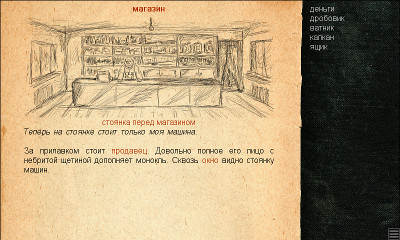
\includegraphics[scale=0.7]{1.jpg}
\caption{INSTEAD с запущенной игрой}
\label{INSTEAD-running}
\end{wrapfigure}

\index{Главное окно}
\textbf{Главное окно} игры содержит информацию о статической и динамической части сцены, активные события и картинку сцены с возможными переходами в другие сцены (в графическом интерпретаторе).

\index{Сцена!динамическая часть}
\textbf{Динамическая часть} сцены составлена из описаний объектов сцены, она отображается всегда. Она может выглядеть так: <<Стоит стол. Рядом стоит стул>>. Если динамическая часть пуста, то игроку не с чем контактировать в сцене.

\index{Сцена!статическая часть}
\textbf{Статическая часть} сцены описывает саму сцену, её <<декорации>>. Она отображается при показе сцены (единожды или каждый раз -- решает автор игры), или при повторении команды look (в графическом интерпретаторе при щелчке на названии сцены).

\index{Инвентарь}
Игрок имеет собственный \textbf{инвентарь}. В нём лежат объекты, доступные на любой сцене. Чаще всего инвентарь рассматривают как некую <<котомку>>, в которой лежат объекты; в этом случае каждый объект считают предметом. Такая трактовка практична, обыденна и интуитивна; но не единственна. Понятие инвентаря является условным, ведь это лишь контейнер. В нём могут находиться такие объекты, как <<открыть>>, <<потрогать>>, <<лизнуть>>. Можно наполнить его объектами <<нога>>, <<рука>>, <<мозг>>. Автор игры свободен в определении этих понятий, но он также должен определить действия игрока над ними.

На рисунке \ref{INSTEAD-running} очень чётко видны границы между этими областями. Главное окно имеет бежевый фон, инвентарь -- чёрный. Динамическая часть идёт сразу после ссылок перехода и выделена курсивом; статическая часть отпечатана обычным шрифтом.

Действиями игрока могут быть:

\begin{itemize}
\item {осмотр сцены}
\item {действие на объект сцены}
\item {действие на объект инвентаря}
\item {действие объектом инвентаря на объект сцены}
\item {действие объектом инвентаря на объект инвентаря}
\end{itemize}

Осмотр сцены -- это чаще всего неявное действие. Игрок входит в комнату, он автоматически осматривает её.

\index{Действие!на объект сцены}
Действие на объект сцены обычно понимается как изучение объекта, или использование его. Например, если в сцене существует объект <<чашка кофе>>, то действием на него может быть выпивание кофе, тщательный осмотр чашки, разбивание чашки или перемещение чашки в инвентарь. Это определяется только автором и никем другим.

\index{Действие!на объект инвентаря}
Действие на объект инвентаря понимается аналогично. Например, если в инвентаре лежит объект <<яблоко>>, его можно съесть или осмотреть. С другой стороны, если в инвентаре лежит объект <<осмотреть>>, то действие над ним будет трудно описать логически.

\index{Действие!объектом на объект}
Действие объектом инвентаря на объект сцены -- это чаще всего использование или передача объекта. Например, действие объектом <<нож>> на объект <<бармен>> может означать передачу ножа бармену, угрозу ножом бармену, убийство ножом бармена и многое другое.

Действие объектом инвентаря на объект инвентаря понимается так же свободно. Это может быть соединение предметов (<<сарделька>> + <<кетчуп>>) в одно (<<сарделька с кетчупом>>), либо использование (<<открыть>> + <<ящик>>).

Эти примеры подробно показывают первую из идей STEAD -- гибкость. Автор свободен в своей фантазии и может трактовать все понятия движка как хочет.

Игра представляет из себя каталог, в котором должен находиться скрипт main.lua. Другие ресурсы игры (скрипты на lua, графика и музыка) должны находиться в рамках этого каталога. Все ссылки на ресурсы делаются относительно текущего каталога -- каталога игры.

Игра начинается именно с main.lua. В начале файла main.lua может быть определён заголовок, состоящий из тегов. Теги должны начинаться с символов комментария \verb/--/. На данный момент существуют два тега: \verb/$Name:,/ который должен содержать название игры, и \verb/$Version:,/который указывает версию игры. Пример использования тега:

\begin{verbatim}
-- $Name: Самая интересная игра!$
\end{verbatim}

После тегов следует указать версию интерпретатора, которую требует игра:

\begin{verbatim}
instead_version "1.3.0"
\end{verbatim}

Если это указание отсутствует, то STEAD будет работать в режиме совместимости, используя устаревшее API. Описание устаревшего API находится в предыдущих версиях данного справочника и убрано из данного издания для краткости.

Интерпретатор ищет доступные игры в следующих каталогах:
\index{Каталоги!игр}

Unix версия интерпретатора просматривает \verb;/usr/local/share/instead/games; (по умолчанию), а также \verb,~/.instead/games,.

Windows сборка использует каталог \verb/куда-вы-установили-INSTEAD\games/.

Расположение пользовательских игр также зависит от вашей версии Windows. Например, в Windows Vista игры могут лежать в каталоге \verb/AppData\Local\instead\games/.

На данный момент активно развивается только графическая ветка интерпретатора -- INSTEAD-SDL. Поэтому справочник в б\'{о}льшей мере описывает её возможности.

\section{Сцена}\index{Сцена}

Сцена -- это единица игры, в рамках которой игрок может изучать все объекты сцены и взаимодействовать с ними. В игре должна быть сцена с именем main.

\begin{verbatim}
main = room {
        nam = 'главная комната',
        dsc = 'Вы в большой комнате.',
};
\end{verbatim}

Отмечу, что пример выше является минимальной игрой для INSTEAD. Это некий <<Hello, World>>, который я рекомендую сохранить под именем main.lua и поместить в отдельную папку в каталоге для игр.

\index{Атрибуты!nam}

Атрибут \verb/nam/ (имя) является необходимым для любого объекта. Для сцены это -- то, что будет заголовком сцены при её отображении. Имя сцены также используется для её идентификации при переходах.

\index{Атрибуты!dsc}
Атрибут \verb/dsc/ -- это описание статической части сцены, которое выводится при входе в сцену или выполнении команды look.

\index{Атрибуты!forcedsc}
\textbf{\textcolor{red}{Внимание!!!}} Если для вашего творческого замысла необходимо, чтобы описание статической части сцены выводилось на каждом ходу (а не только при первом входе в сцену), вы можете определить для своей игры параметр forcedsc (в начале игры).

\begin{verbatim}
game.forcedsc = true;
\end{verbatim}

Или, аналогично, задать атрибут forcedsc для конкретных сцен.

\index{[[ ]]}
Для длинных описаний удобно использовать запись вида:

\begin{verbatim}
dsc = [[ Очень длинное описание... ]],
\end{verbatim}

При этом переводы строк игнорируются. Если вы хотите, чтобы в выводе описания сцены присутствовали абзацы -- используйте символ \verb/^/.

\begin{verbatim}
dsc = [[ Первый абзац. ^^
Второй Абзац.^^

Третий абзац.^
На новой строке.]],
\end{verbatim}

Символы \verb/^/ и \verb/|/ можно экранировать в строках, если вы хотите их напечатать для пользователя:

\begin{verbatim}
 p " \\^ \\| "
 p [[ \^ \| ]]
\end{verbatim}

К текущей сцене можно обратиться через функцию \verb/here()/.
\index{Функции!here}

\section{Объект}
\index{Объекты!нормальные}
\subsection{Нормальные объекты}
Объекты -- это единицы сцены, с которыми взаимодействует игрок.

\begin{verbatim}
table = obj {
        nam = 'стол',
        dsc = 'В комнате стоит {стол}.',
        act = 'Гм... Просто стол...',
};
\end{verbatim}

Имя объекта \verb/nam/ используется для адресации объекта.

\index{Атрибуты!dsc}
\verb/dsc/ -- описатель объекта. Он будет выведен в динамической части сцены. Фигурными скобками отображается фрагмент текста, который будет являться ссылкой в графическом интерпретаторе. Если вы забудете сделать ссылку, то интерпретатор не выдаст ошибки, но игроки не смогут взаимодействовать с объектом.

\index{Атрибуты!act}
\verb/act/ -- это обработчик, который вызывается при действии пользователя на объект сцены. Если объект находится в инвентаре, то действие с ним будет передаваться другому обработчику -- \verb/inv/.

До сих пор в примерах приводились примитивные обработчики, которые всего лишь возвращают определённую строку. В примере выше обращение к объекту вызовет банальную реакцию: интерпретатор напечатает строку <<Гм... Просто стол...>>. Хуже того: он будет отвечать тем же образом каждый раз при обращении к объекту. Это не совсем гибкий подход, поэтому STEAD позволяет определить любой атрибут объекта как функцию. Так, возможно построить такую конструкцию:

\begin{verbatim}
apple = obj {
        nam = 'яблоко',
        dsc = function(s)
                if not s._seen then
                        return 'На столе {что-то} лежит.';
                else
                        return 'На столе лежит {яблоко}.';
                end
        end,
        act = function(s)
                if s._seen then return 'Это яблоко!';
                else
                        s._seen = true;
                        return 'Я присматриваюсь и понимаю, что это -- яблоко.!';
                end
        end,
};
\end{verbatim}

\index{Функции}
Если атрибут или обработчик оформлен как функция, то обычно первый аргумент функции \verb/(s)/ есть сам объект. В данном примере, при показе сцены будет в динамической части сцены будет текст: <<На столе что-то лежит>>. При взаимодействии со ссылкой <<что-то>>, переменная \verb/_seen/ объекта \verb/apple/ будет установлена в \verb/true/, и мы увидим, что это было яблоко.

\index{Переменные}
Запись \verb/s._seen/ означает, что переменная \verb/_seen/ размещена в объекте \verb/s/ (то есть, \verb/apple/). В языке Lua переменные необязательно объявлять заранее, при первом обращении к ней переменная \verb/apple._seen/ появится сама; но хорошим тоном будет заранее \textbf{проинициализировать} переменную со значением \verb/false/.

Подчёркивание в имени переменной означает, что она \textbf{попадёт} в файл сохранения игры. Сохраняются все переменные, название которых начинается с с подчёркивания.

Вы можете переопределить функцию \verb/isForSave(k)/, если вас это не устраивает, либо (рекомендованный вариант) воспользоваться блоком \verb/var/, в котором сохраняются все переменные. Для краткости примеры этого руководства не следят за сохранением переменных.

\textbf{\textcolor{red}{Внимание!!!}} Переменные в любом случае не записываются в файл сохранения, если они не размещены в одном из перечисленных типов объектов: комната, объект, диалог, игра, игрок, глобальное пространство.

В файл сохранения могут быть записаны строки, числа, логические значения, ссылки на объекты и конструкции \verb/code/ (о них чуть ниже).

Также вы можете определять переменные при помощи блоков \verb/var/ и \verb/global/, о которых будет рассказано позже.

Рассмотрим другой пример:

\begin{verbatim}
button = obj {
  nam = "кнопка",
  dsc = "На стене комнаты видна большая красная {кнопка}.",
  act = code[[ p 'Я нажал на кнопку.' ]]
}
\end{verbatim}

Здесь я использовал две новых конструкции: \verb/code/ и \verb/p/. Конструкция \verb/code [[ код ]]/ - это короткая форма записи для:

\begin{verbatim}
act = function(self, ...)
 код
end,
\end{verbatim}

При этом внутри \verb/code/ определены переменные \verb/self/ -- текущий объект, \verb/arg1/, \verb/arg2/, ..., \verb/arg9/ -- параметры функции, и массив параметров \verb/args[]./

Также для сокращения записи нужна функция \verb/p/. Она возвращает текст, заканчивая его пробелом. Всего определено три подобных функции:

\begin{description}
\item[p] -- выводит переданный текст, заканчивая его пробелом
\item[pn] -- выводит переданный параграф, заканчивая его переводом строки
\item[pr] -- выводит переданное как есть
\end{description}

Lua позволяет опускать скобки вокруг параметров, если параметр всего один.

Если необходимо показать, что действие невыполнимо, можно вернуть из обработчика значение \verb/false/ или \verb/nil/. При этом будет отображено описание по умолчанию -- так, для обработчика \verb/act/ это будет  \verb`game.act.`

Если обработчик не возвращает ничего, то он выполняется, а отображается описание по умолчанию.

\subsection{Облегчённые объекты}

\index{Объекты!облегчённые}
Иногда, сцену нужно наполнить декорациями, которые обладают ограниченной функциональностью, но делают игру разнообразней. Для этого можно использовать облегчённый объект. Например:

\begin{verbatim}
sside = room {
        nam = 'южная сторона',
        dsc = [[Я нахожусь у южной стены здания института. ]],
        act = function(s, w)
                if w == "подъезд" then
                        ways():add('stolcorridor');
                        return "Я подошёл к подъезду. Хм -- зайти внутрь?";
                end
        end,
        obj = {vobj("подъезд", "Я вижу небольшой {подъезд}.")},
};
\end{verbatim}

\index{Объекты!облегчённые!vobj}
Как видим, \verb/vobj/ позволяет сделать лёгкую версию статического объекта, с которым тем не менее можно взаимодействовать (за счёт определения обработчика \verb/act/ в сцене и анализа ключа объекта). \verb/vobj/ также вызывает метод \verb/used/, при этом в качестве третьего параметра передаётся объект, воздействующий на виртуальный объект.

Синтаксис \verb/vobj/ таков: \verb/vobj(имя, описатель)./

\index{Объекты!облегчённые!vway}
Существует модификация объекта \verb/vobj/ под именем \verb/vway/. \verb/vway/ реализует ссылку. Синтаксис и пример:

\begin{verbatim}
vway(имя, описание, сцена назначения);
obj = { vway("дальше", "Нажмите {здесь}.", 'nextroom') }
\end{verbatim}

Вы можете динамически заполнять сцену объектами \verb/vobj/ или \verb/vway/ с помощью методов \verb/add/ и \verb/del/.

\index{Объекты!облегчённые!vroom}
В довершение, определена также упрощённая сцена \verb/vroom/. Синтаксис:

\begin{verbatim}
vroom(имя перехода, сцена назначения)
\end{verbatim}

Ниже приводится несколько примеров и трюков с подобными объектами:

\begin{verbatim}
home.objs:add(vway("next", "{Дальше}.", 'next_room');
home.objs:del("next");
home.objs:add(vroom("идти на запад", 'mountains');
if not home.obj:srch('Дорога') then
 home.obj:add(vway('Дорога', 'Я заметил {дорогу} в лес.', 'forest'));
end
obj = {vway('Дорога', 'Я заметил {дорогу} в лес.', 'forest'):disable()},
objs()[1]:disable();
objs()[1]:enable();
\end{verbatim}

\subsection{Динамическое создание объектов}
\index{Функции!new}
\index{Функции!delete}
Вы можете использовать аллокаторы \verb/new/ и \verb/delete/ для создания и удаление динамических объектов:

\begin{verbatim}
new("obj { nam = 'a' ..... }")
put(new [[obj {nam = 'test' } ]]);
put(new('myconstructor()');
\end{verbatim}

Созданный объект будет попадать в файл сохранения. \verb/new()/ возвращает реальный объект; чтобы получить его имя, если это нужно, используйте функцию \index{Функции!deref} \verb/deref()./

\section{Некоторые манипуляции с объектами}

\subsection{Объект и сцена}

\index{Ссылки!на объект}
Ссылкой на объект называется текстовая строка, содержащая имя объекта при его создании.

Например: \verb/'table'/ -- ссылка на объект \verb/table/.

\index{Атрибуты!obj}
Для того, чтобы поместить в сцену объекты, нужно определить массив \verb/obj/, состоящий из ссылок на объекты:

\begin{verbatim}
main = room {
        nam = 'главная комната',
        dsc = 'Вы в большой комнате.',
        obj = { 'tabl' },
};
\end{verbatim}

\subsection{Объекты, связанные с объектами}

\index{Объекты!связанные}
\index{Атрибуты!obj}

Объекты тоже могут содержать атрибут \verb/obj./ При этом, список будет последовательно разворачиваться. Например, поместим на стол яблоко:

\begin{verbatim}
apple = obj {
        nam = 'яблоко',
        dsc = 'На столе лежит {яблоко}.',
};

table = obj {
        nam = 'стол',
        dsc = 'В комнате стоит {стол}.',
        obj = { 'apple' },
};
\end{verbatim}

При этом, в описании сцены мы увидим описание объектов <<стол>> и <<яблоко>>, так как \verb/apple/ -- связанный с \verb/table/ объект.

\subsection{Действия объектов друг на друга}

\index{Действие!объектом на объект}
Игрок может действовать объектом инвентаря на другие объекты. При этом вызывается обработчик \verb/use/ у объекта которым действуют и \verb/used/ -- на которого действуют.

Например:

\begin{verbatim}
knife = obj {
        nam = 'нож',
        dsc = 'На столе лежит {нож}',
        inv = 'Острый!',
        tak = 'Я взял нож!',
        use = 'Вы пытаетесь использовать нож.',
};

tabl = obj {
        nam = 'стол',
        dsc = 'В комнате стоит {стол}.',
        act = 'Гм... Просто стол...',
        obj = { 'apple', 'knife' },
        used = 'Вы пытаетесь сделать что-то со столом...',
};
\end{verbatim}

Если игрок возьмёт нож и использует его на стол, то увидит текст обработчиков \verb/knife.use/ и \verb/tabl.used/.

\verb/use/ и \verb/used/ могут быть функциями. Тогда первый параметр это сам объект, а второй -- ссылка на объект, на который направлено действие в случае \verb/use/ и объект, которым действие осуществляется в случае \verb/used/.

\verb/use/ может вернуть статус \verb/false/, в этом случае обработчик \verb/used/ не вызывается (если он вообще был). Статус обработчика \verb/used/ -- игнорируется. Это будет выглядеть как:

\begin{verbatim}
return 'Строка реакции', false;
\end{verbatim}

Возможно также действовать объектами сцены на объекты сцены; для этого нужно установить переменную \verb/game.scene_use = true/ или поставить \verb/scene.use=true/ в нужной комнате. В этом случае использование объектов сцены будет аналогично использованию объектов инвентаря.

\subsection{Скрытие объектов}

\index{Объекты!скрытые}
\index{Методы!enable}
\index{Методы!disable}

При помощи методов \verb/enable/ и \verb/disable/ становится возможным управлять появлением и исчезновением объектов.

Скрытый объект -- это объект, который находится в сцене, но на данный момент словно бы <<выключен>>. Он присутствует для движка, но не существует для игрока. Его описание не выводится и с ним невозможно контактировать. Это можно использовать, например, вместо динамического создания объектов.

Чтобы создать заведомо выключенный объект, необходимо воспользоваться конструкцией вида:

\begin{verbatim}
knife = {<...>}:disable()
\end{verbatim}

Объект \verb/knife/ будет создан и тут же выключен.

Методы \verb/enable()/ и \verb/disable()/ возвращают сам объект. Они присутствуют у любого объекта и списка объектов.

\section{Смена сцен}

\index{Сцена!смена сцен}

Как только главный герой уходит со сцены, декорации меняются. Но чтобы игрок ушёл из нашей сцены, он должен знать, куда идти.

\index{Атрибуты!way}
Для перехода между сценами используется атрибут сцены -- список \verb/way/.

\begin{verbatim}
room2 = room {
        nam = 'зал',
        dsc = 'Вы в огромном зале.',
        way = { 'main' },
};

main = room {
        nam = 'главная комната',
        dsc = 'Вы в большой комнате.',
        obj = { 'tabl' },
        way = { 'room2' },
};
\end{verbatim}

При этом, вы сможете переходить между сценами \verb/main/ и \verb/room2/. Как вы помните, \verb/nam/ может быть функцией, и вы можете генерировать имена сцен на лету, например, если вы хотите, чтобы игрок не знал название сцены, пока не попал на неё.

\index{Атрибуты!exit}
\index{Атрибуты!enter}
\index{Атрибуты!left}
\index{Атрибуты!entered}
При переходе между сценами движок вызывает обработчик \verb/exit/ из текущей сцены и \verb/enter/ той сцены, куда идёт игрок. \verb/exit/ и \verb/enter/ могут быть функциями -- тогда первый параметр это сам объект, а второй -- ссылка на комнату куда игрок хочет идти (для \verb/exit/) или из которой уходит (для \verb/enter/).

После перехода вызываются обработчики \verb/left/ прошлой сцены и \verb/entered/ сцены, куда перешёл игрок.

Например:

\begin{verbatim}
room2 = room {
        enter = function(s, f)
                if f == main then
                        return 'Вы пришли из комнаты.';
                end
        end,
        nam = 'зал',
        dsc = 'Вы в огромном зале.',
        way = { 'main' },
        exit = function(s, t)
                if t == main then
                        return 'Я не хочу назад!', false
                end
        end,
};
\end{verbatim}

\index{Атрибуты!tak}
Как видим, обработчики могут возвращать два значения: строку и статус. В нашем примере функция \verb/exit/ вернёт \verb/false/, если игрок попытается уйти из зала в \verb/main/. \verb/false/ блокирует переход. Такая же логика работает и для \verb/enter/. Кроме того, она работает и для обработчика \verb/tak/ (о нём чуть позже).

\index{Функции!goto}
Если требуется перейти на другую сцену автоматически, можно использовать функцию \verb/goto/ со ссылкой на сцену как параметром:

\begin{verbatim}
return goto('main');
goto('main');
\end{verbatim}

\section{Специальные типы объектов}

\subsection{Инвентарь}

\index{Инвентарь}
\index{Функции!inv}

Инвентарь проще всего возвращается функцией inv(). Он представлен списком, поэтому для него справедливы все их трюки (см. соответствующий раздел).

\index{Функции!tak}
Простейший вариант сделать объект, который можно брать -- определить у него обработчик tak.

Если предмет сцены имеет обработчик \verb/tak/ и НЕ имеет обработчика \verb/act/ \footnote{Пользуясь случаем: я считаю, что tak -- немного неудобное имя. Именно так. -- А.Я.}, то при действии на нём вызывается не \verb/act/, а \verb/tak/; после этого предмет перемещается в инвентарь. Это происходит вот так:

\begin{verbatim}
apple = obj {
        nam = 'яблоко',
        dsc = 'На столе лежит {яблоко}.',
        tak = 'Вы взяли яблоко.',
};
\end{verbatim}

\subsection{Игрок}

\index{Объекты!pl}
Игрок в STEAD представлен объектом \verb/pl/. Тип объекта -- \verb/player/.

\index{Атрибуты!obj}
Атрибут \verb/obj/ представляет собой инвентарь игрока.

Объекты игрока можно воспринимать как объекты инвентаря, в этом случае верны следующие конструкции:

\begin{verbatim}
remove('knife', me());
put('knife', me());
take('knife', me());
where('knife');
\end{verbatim}

Необходимо отметить, что это верно не в каждой игре.

\subsection{Игра}

\index{Объекты!game}
Игра представлена объектом \verb/game/. Он хранит в себе указатель на текущего игрока (\verb/'pl'/) и некоторые параметры. Например, вы можете указать в начале своей игры кодировку текста следующим образом:

\begin{verbatim}
game.codepage="UTF-8";
\end{verbatim}

\index{Атрибуты!act}
\index{Атрибуты!inv}
\index{Атрибуты!use}
Кроме того, объект \verb/game/ может содержать обработчики по умолчанию \verb/act/, \verb/inv/, \verb/use/, которые будут вызваны, если в результате действий пользователя не будут найдены никакие другие обработчики. Например, вы можете написать в начале игры:

\begin{verbatim}
game.act = 'Не получается.';
game.inv = 'Гм.. Странная штука..';
game.use = 'Не сработает...';
\end{verbatim}

На практике полезно что-то вроде:

\begin{verbatim}
game.inv = function()
 local reaction = {
  [1] = 'Либо я ошибся карманом, либо мне нужно что-то другое.',
  [2] = 'Откуда у меня в кармане ЭТО?!',
  [3] = 'Сам не понял, что достал. Положу обратно.',
  [4] = 'Это что-то неправильное.',
  [5] = 'В моих карманах что только не залёживается...',
  [6] = 'Я не представляю, как я могу тащить ЭТО с собою.',
  [7] = 'Мне показалось или оно на меня смотрит?',
 };
 return reaction[rnd(#reaction)];
end;
\end{verbatim}

\subsection{Таймер}
\index{Объекты!timer}
\label{objects_timer}
Таймер -- это объект \verb/timer/, который служит для отсчёта \textbf{реального} времени (в миллисекундах). В этом его существенное отличие от атрибутов \verb/life/, которые служат для измерения игрового времени (в шагах).

Для управления таймером используются функции:

\begin{description}
\item[timer:set(ms)] задать интервал таймера в миллисекундах
\item[timer:stop()] отключить таймер
\item[timer.callback(s)] функция-обработчик таймера, которая вызывается через заданный интервал времени
\end{description}

Двоеточия при вызове \verb/set/ и \verb/stop/ важны, их не стоит заменять на точки. По умолчанию таймер выключён, и не имеет заданного обработчика. Если таймер включён, то обработчик вызывается с заданным интервалом.

Чтобы включить таймер после выполнения \verb/stop/, достаточно переинициализировать его командой \verb/set/ с прежним интервалом.

Пример использования таймера:

\begin{verbatim}
timer.callback = function(s)
 main.time = main.time + 1;
 return "look";
end
timer:set(100);

main = room {
 time = 1,
 forcedsc = true,
 nam = 'Таймер',
 dsc = function(s)
  return 'Демонстрация: '..tostring(s._time);
 end
};
\end{verbatim}

\subsection{Ввод с клавиатуры}
\index{Объекты!input}
\label{objects_input}
Ввод с клавиатуры анализируется при помощи объекта \verb/input/. Этот объект принимает все нажатия клавиш. По умолчанию он не имеет запрограммированных обработчиков, поэтому ничего не выполняет.

Создание нового обработчика для клавиши выполняется командой \verb/input.key(s, pressed, key),/ где \verb/pressed/ -- нажатие или отжатие, \verb/key/ -- символьное имя клавиши;

Если обработчик возвращает не \verb/nil/, то клавиша обрабатывается \textbf{им}, а не интерпретатором. Таким образом, можно переопределить обработку любой клавиши.

Например:

\begin{verbatim}
input.key = function(s, pr, key)
 if not pr or key == "escape" then return
 elseif key == 'space' then key = ' '
 elseif key == 'return' then key = '^';
 end
 if key:len() > 1 then return end
 main.txt = main.txt:gsub('_$','');
 main.txt = main.txt..key..'_';
 return "look";
end

main = room {
 txt = '_',
 forcedsc = true,
 nam = 'Клавиатура',
 dsc = function(s)
  return 'Демонстрация: '..tostring(s._txt);
 end
};
\end{verbatim}

\section{Диалоги}

\index{Диалоги}

Третьим важным типом в движке являются диалоги. Диалоги -- это особый подвид сцен, содержащий только фразы. Например, диалог может выглядеть следующим образом:

\begin{verbatim}
povardlg = dlg {
 nam = 'на кухне',
 dsc = 'Передо мной полное лицо повара...',
 obj = {
  [1] = phr('Мне вот-этих зелёненьких... Ага - и бобов!', 'На здоровье!'),
  [2] = phr('Картошку с салом, пожалуйста!', 'Приятного аппетита!'),
  [3] = phr('Две порции чесночного супа!!!', 'Прекрасный выбор!'),
  [4] = phr('Мне что-нибудь лёгонькое, у меня язва...', 'Овсянка!'),
 },
};
\end{verbatim}

\index{Функции!phr}
\verb/phr/ -- создание фразы. Фраза содержит вопрос, ответ и реакцию (реакция в данном примере отсутствует). Когда игрок выбирает одну из фраз, фраза отключается. Когда все фразы отключатся диалог заканчивается. Реакция -- это строка кода на lua который выполнится после отключения фразы.

\index{Функции!\_phr}
\verb/_phr/ -- создание выключенной фразы. Она не видна изначально, но её можно включить с помощью функции \verb/pon()/ (см. ниже). По смыслу это эквивалентно \verb/phr(<...>):disable()./

Вот как создаётся фраза:

\begin{verbatim}
[1] = phr('Можно задать вопрос?', 'Конечно!', [[pon(1);]]),
\end{verbatim}

В реакции может быть любой lua код (простейшей реакцией является возвращение строки), но в STEAD определены наиболее часто используемые функции:

\index{Функции!pon}
\index{Функции!poff}
\index{Функции!prem}
\index{Функции!pseen}
\index{Функции!punseen}
\begin{description}
\item[pon(n...)] включить фразы диалога с номерами n... (в нашем примере -- чтобы игрок мог повторно взять еду того-же вида).
\item[poff(n...)] выключить фразы диалога с номерами n...
\item[prem(n...)] удалить (заблокировать) фразы диалога с номерами n... Удаление означает невозможность включения фраз. \verb/pon(n..)/ не приведёт к включению фраз.
\item[pseen(n...)] вернет true, если все заданные фразы диалога видимы.
\item[punseen(n...)] вернет true, если все заданные фразы диалога невидимы.
\end{description}

Если параметр \verb/n/ не указан, действие относится к текущей фразе.

Как ответ, так и реакция могут быть функциями. Вы можете закончить диалог, выполнив в реакции функцию \verb/back()./

Переход в диалог осуществляется как переход на сцену:

\begin{verbatim}
return goto('povardlg');
\end{verbatim}

Вы можете переходить из одного диалога в другой диалог -- организовывая иерархические диалоги.

Также, вы можете прятать некоторые фразы при инициализации диалога и показывать их при некоторых условиях.

\index{Методы!pon}
\index{Методы!poff}
Вы можете включать/выключать фразы не только текущего, но и произвольного диалога, с помощью методов объекта диалог \verb,pon/poff,. Например:

\begin{verbatim}
shopman:pon(5);
\end{verbatim}

Если номер фразы не указан, то это означает, что действие относится к текущей фразе:

\begin{verbatim}
phr('a', 'b', [[ pon() ]]);
\end{verbatim}

\index{Методы!empty}
У самих диалогов также есть метод \verb/empty/. С его помощью можно проверять, пуст ли диалог:

\begin{verbatim}
if dlg:empty() then p "Диалог пуст" end
\end{verbatim}

\section{О списках}

Каждый атрибут-список имеет методы:

\begin{description}
\item[add] \index{Методы!add} Добавление элемента в список. Необязательным вторым параметром является позиция в списке.
\item[del] \index{Методы!del} Удаление элемента из списка. Выключённые элементы не удаляются.
\item[purge] \index{Методы!purge} Удаление элемента из списка. Выключённые элементы также удаляются.
\item[look] \index{Методы!look} Получение индекса элемента в списке по идентификатору
\item[srch] \index{Методы!srch} Проверка на наличие объекта в списке по его nam. Возвращает 2 значения: идентификатор и позицию; если объекта нет, вернёт nil. Например: \begin{verbatim}objs():srch('Ножик')\end{verbatim}
\item[replace] \index{Методы!replace} Замена объекта в списке другим
\item[set] \index{Методы!set} Изменение объекта по номеру. Например, этот пример присвоит заменит первый объект списка: \begin{verbatim}objs():set('knife',1);\end{verbatim}
\item[disable] \index{Методы!disable} Скрытие объекта в списке; отличается от удаления тем, что может быть возвращён к жизни через метод enable
\item[enable] \index{Методы!enable} Показ скрытого объекта
\item[zap] \index{Методы!zap} Обнуление списка
\item[cat(b)] \index{Методы!cat} Склеивает список со списком b
\item[cat(b,pos)] Добавляет в список список b на позицию pos
\item[disable\_all] \index{Методы!disable\_all} Аналогично disable, но массово
\item[enable\_all] \index{Методы!enable\_all} Аналогично enable, но массово
\end{description}

Параметрами методов могут быть объекты, их идентификаторы и имена.

\section{Функции}
Замечание. Если аргумент у функции единственен и текстовый, то скобки вокруг аргумента можно опускать. Большинство описываемых в этом разделе функций с несколькими параметрами могут
использоваться без указания всех параметров. В этом случае опущенные параметры принимают значение по умолчанию (обычно -- текущая сцена).
.
\begin{description}
\item[inv()] \index{Функции!inv} возвращает список инвентаря
\item[objs()] \index{Функции!objs} возвращает список объектов указанной сцены; если сцена не указана, то возвращает список объектов текущей сцены.
\item[ways()] \index{Функции!ways} возвращает список возможных переходов из  указанной сцены; если сцена не указана, то возвращает список возможных переходов из  текущей сцены.
\item[me()] \index{Функции!me} возвращает объект pl (объект игрока)
\item[here()] \index{Функции!here} возвращает текущую сцену
\item[where()] \index{Функции!where} возвращает сцену в которой помещен объект (если он был добавлен с использованием функций put, drop, move)
\item[from()] \index{Функции!from} возвращает прошлую сцену
\item[ref(nam)] \index{Функции!ref} возвращает указанный объект: \begin{verbatim}ref('home') == home\end{verbatim} nam может быть функцией, строкой или текстовой ссылкой
\item[deref(object)] \index{Функции!deref} возвращает ссылку строкой для объекта: \begin{verbatim}deref(knife) == 'knife'\end{verbatim}
\item[nameof(object)] \index{Функции!nameof} возвращает \verb/nam/ объекта
\item[have(object)] \index{Функции!have} проверяет, есть ли объект в инвентаре по имени объекта или по его nam
\item[move(from, where, to)] \index{Функции!move} переносит объект из текущей сцены в другую
\item[movef(from, where, to)] \index{Функции!movef} действует так же, но добавляет объект в начало списка
\item[moveto(from,where,to,position)] \index{Функции!moveto} перемещает элемент в нужную позицию списка объектов
\item[seen(object,scene)] \index{Функции!seen} проверяет, есть ли объект в указанной сцене (в текущей, если сцена не указана)
\item[exist(object,scene)] \index{Функции!exist} делает то же самое, что и \verb/seen/, но учитывает и выключенные объекты
\item[path(scene,scene)] \index{Функции!path} проверяет, есть ли путь в нужную сцену из указанной
\item[drop(object,scene)] \index{Функции!drop} выбрасывает объект из инвентаря в указанную сцену (в текущую, если сцена не указана)
\item[dropf(object,scene)] \index{Функции!dropf} то же, что drop, но объект появляется в начале списка
\item[dropto(object,scene,position)] \index{Функции!dropto} выбрасывает объект на нужную позицию
\item[put(object,scene)] \index{Функции!put} кладёт предмет в указанную сцену; в текущую, если сцена не указана
\item[putf(object,scene)] \index{Функции!putf} кладёт предмет в начало списка
\item[putto(object,scene,position)] \index{Функции!putto} кладёт предмет в указанную позицию списка
\item[remove(object,scene)] \index{Функции!remove} удаляет предмет из указанной сцены; из текущей, если сцена не указана
\item[take(object,scene)] \index{Функции!take} перемещает объект из указанной(текущей) сцены в инвентарь
\item[takef(object)] \index{Функции!takef} берёт объект в инвентарь на первую позицию
\item[taketo(object,position)] \index{Функции!taketo} берёт объект в инвентарь на указанную позицию
\item[taken(object)] \index{Функции!taken} проверяет, взят ли уже объект
\item[rnd(m)] \index{Функции!rnd} возвращает случайное целое значение от 1 до m
\item[goto(destination)] \index{Функции!goto} переносит в сцену w; используется в конструкции вида \verb/return goto('inmycar');/
\item[change\_pl(player)] \index{Функции!change\_pl} переключает на другого игрока (со своим инвентарём и позицией), также используется в \linebreak \verb/return/. Может использоваться для переключения между разными инвентарями.
\item[back()] \index{Функции!back} переносит в предыдущую сцену (аналогично goto)
\item[time()] \index{Функции!time} возвращает текущее время игры в активных действиях.
\item[cat(...)] \index{Функции!cat} возвращает строку -- склейку строк-аргументов. Если первый аргумент nil, то функция возвращает nil.\footnote{Функция легко и просто заменяется обычным оператором склейки строк Lua: \texttt{строка1 .. строка2}. Тем не менее, этот оператор выдаст ошибку при склейке nil}
\item[par(...)] \index{Функции!par} возвращает строку -- склейку строк-аргументов, разбитых строкой-первым параметром.
\end{description}

Следующие записи эквивалентны:

\begin{verbatim}
ref('home').obj:add('chair');
home.obj:add('chair');
objs('home'):add('chair');
put('chair', 'home');
\end{verbatim}

Если вы хотите перенести объект из произвольной сцены, вам придётся удалить его из старой сцены с помощью метода del. Для создания сложно перемещающихся объектов, вам придётся написать свой метод, который будет сохранять текущую позицию объекта в самом объекте и делать удаление объекта из старой сцены. Вы можете указать исходную позицию (комнату) объекта в качестве третьего параметра move.

\begin{verbatim}
move('mycat','inmycar', 'forest');
\end{verbatim}

Отдельно следует упомянуть функции альтернативного вывода текста. Их назначение можно понять по следующим формам записи:

\begin{verbatim}
act = function(s)
       p "Я осмотрел его...';
       p "Гммм...."
end

act = function(s)
       return "Я осмотрел его... Гммм...."
end
\end{verbatim}

\begin{description}
\item[p] \index{Функции!p} Добавляет строку и пробел в буфер
\item[pn] \index{Функции!pn} Добавляет строку и перевод строки в буфер
\item[pclr] \index{Функции!pclr} Очистка буфера
\item[pget] \index{Функции!pget} Получение содержимое буфера на текущий момент
\end{description}

Другой пример:

\begin{verbatim}
life = function(s)
     p 'Ветер дует мне в спину.'
     return pget(), true
end
\end{verbatim}

\section{Добавление динамики в игру}
\index{Атрибуты!life}

Игра измеряет время в своих единицах -- в шагах, или активных действиях. Каждое действие игрока -- это его шаг, пусть даже он тратит его на то, чтобы ещё раз осмотреться. Что он увидит нового? Что изменится в мире игры за это время?

Именно для того, чтобы задать динамику мира, существует система с говорящим названием life.

Вы можете определять обработчики, которые выполняются каждый раз, когда время игры увеличивается на 1. Например:

\begin{verbatim}
mycat = obj {
        nam = 'Барсик',
        lf = {
                [1] = 'Барсик шевелится у меня за пазухой.',
                [2] = 'Барсик выглядывает из за пазухи.',
                [3] = 'Барсик мурлычет у меня за пазухой.',
                [4] = 'Барсик дрожит у меня за пазухой.',
                [5] = 'Я чувствую тепло Барсика у себя за пазухой.',
        },
        life = function(s)
                local r = rnd(5);
                if r > 2 then
                        return;
                end
                r = rnd(5);
                return s.lf[r];
        end,
\end{verbatim}

\index{Функции!lifeon}
В этом примере кот по имени Барсик, сидя в инвентаре у игрока, будет на каждом шагу показывать свою активность. Но приведённый код пока что не будет работать. Для того, чтобы объявить объект <<живым>>, следует добавить его в соответствующий список с помощью функции \verb/lifeon()/.

\begin{verbatim}
 inv():add('mycat');
 lifeon('mycat');
\end{verbatim}

\index{Функции!lifeoff}
Любой объект или сцена могут иметь свой обработчик \verb/life/, который вызывается каждый раз при смене текущего времени игры, если объект или сцена были добавлены в список живых объектов с помощью \verb/lifeon/. Не забывайте удалять живые объекты из списка с помощью \verb/lifeoff/, когда они больше не нужны. Это можно сделать, например, в обработчике \verb/exit/, или любым другим способом.

Вы можете вернуть из обработчика life второй код возврата, важность. (true или false). Если он равен true, то возвращаемое значение будет выведено ДО описания объектов; по умолчанию значение равно false.

\index{Переменные!ACTION\_TEXT}
Если вы хотите <<очистить экран>>, то можно воспользоваться следующим хаком. Из метода \verb/life/ доступна переменная \verb/ACTION_TEXT/ -- это тот текст, который содержит реакцию на действие игрока. Соответственно, сделав \verb/ACTION_TEXT = nil/, можно <<запретить>> вывод реакции. Например, для перехода на конец игры можно сделать:

\begin{verbatim}
ACTION_TEXT = nil
return goto('theend'), true
\end{verbatim}

Также для добавления динамики в игру служат объекты timer и input, см. разделы \ref{objects_timer} и \ref{objects_input}.

\section{Краски и звуки}

В чём очевидное преимущество графического интерпретатора над текстовой веткой -- это то, что он может говорить и показывать. Проще говоря, вы можете добавить в игру графику и музыку.

\index{Атрибуты!pic}
\index{Атрибуты!disp}
Графический интерпретатор анализирует атрибут сцены \verb/pic/, и воспринимает его как путь к картинке-ил\-лю\-страции для сцены. Если в текущей сцене не определён атрибут \verb/pic/, то берётся \verb/game.pic/. Если не определён и он, то картинка не отображается.

Unix-версия движка поставляется в исходных кодах, поэтому поддержка форматов графики и музыки в основном определяется возможностями библиотеки SDL, установленной в вашей системе. В большинстве случаев обеспечивается поддержка всех основных форматов. Для графики я рекомендую использовать форматы PNG, JPG и GIF (также поддерживаются анимированные GIF). Новые версии движка поддерживают GIF-анимацию. Те же правила действуют для музыки. Здесь строгих рамок нет, поэтому старайтесь не использовать редких форматов. Проверена поддержка WAV, MP3, OGG, FLAC, XM, MOD, IT, S3M.

\index{Функции!img}
Вы также можете встраивать графические изображения в текст или в инвентарь с помощью функции \verb/img/. Например:

\begin{verbatim}
knife = obj {
        nam = 'Нож'..img('img/knife.png'),
}
\end{verbatim}

Чтобы разделить иллюстрацию и описание предмета, можно задать иллюстрацию в атрибуте \verb/disp/:

\begin{verbatim}
knife = obj {
 nam = 'Нож';
 disp = img('img/knife.png'),
}
\end{verbatim}

Тогда игра будет обращаться к предмету как \verb/'нож'/, но игроку каждый раз вместо названия предмета будет показываться его иллюстрация.

При этом изображения можно комбинировать, накладывая друг на друга. Очень удобны в этом отношении PNG и GIF, потому что они позволяют задать прозрачность фона.
В случае анимированных GIF наложение происходит только с первым кадром.
Это выглядит следующим образом:

\begin{verbatim}
pic = "gfx/mycat.png;gfx/milk.png@100,100;gfx/fish.png@c20,20"
\end{verbatim}

Картинки складываются стопкой снизу вверх. Самая первая картинка является фоном. Она должна быть самой большой; её границы - это и границы всей картинки.
Точка с запятой разделяет изображения; после неё идёт сначала путь к картинке, затем символ \verb/@/ и координаты точки фона, куда будет помещён левый верхний угол накладываемой картинки.
Координаты считаются от левого верхнего угла фонового изображения. Если после символа \verb/@/ идёт буква \verb/c/, то в эту точку будет помещён не левый верхний угол, а \textbf{центр} накладываемой картинки.

\index{Функции!imgr}
\index{Функции!imgl}
Для того, чтобы вставить картинку у определённого края, нужно вызвать функцию \verb/imgl()/ или \verb/imgr()/. Такие картинки не могут быть ссылками.

Также можно использовать псевдофайлы:

Псевдофайл \verb/pad/ задаёт отступы в изображении:

\verb/imgl 'pad:16,picture.png'/ -- отступы по 16 пикселов от каждого края

\verb/imgl 'pad:0 16 16 4,picture.png'/ -- вверху 0, справа 16, внизу 16, слева 4

\verb/imgl 'pad:0 16,picture.png'/ -- вверху 0, справа 16, внизу 0, слева 16

Псевдофайл \verb/blank/ рисует пустое изображение:

\begin{verbatim}
dsc = img 'blank:32x32'..[[Строка с пустым изображением.]];
\end{verbatim}

Псевдофайл box рисует квадрат. Вы задаёте его размер, цвет и прозрачность (от 0 до 255):

\begin{verbatim}
dsc = img 'box:32x32,red,128'..[[Красный полупрозрачный квадрат.]];
\end{verbatim}

Теперь о звуке. Фоновая музыка задаётся с помощью функции:\index{Функции!set\_music}

\begin{verbatim}
set_music(имя музыкального файла, количество проигрываний)
\end{verbatim}

Она проигрывается циклически бесконечно, если количество проигрываний не задано.

\index{Функции!get\_music} \verb/get_music()/ возвращает текущее имя трека.

\index{Функции!get\_music\_loop} Функция \verb/get_music_loop/ возвращает текущий счетчик проигрываний мелодии. 0 -- означает вечный цикл. n -- количество оставшихся проигрываний. -1 -- проигрывание текущего трека закончено.

\index{Функции!set\_sound}
\index{Функции!get\_sound}
Помимо фонового сопровождения, \verb/set_sound()/ позволяет проиграть звуковой файл. \verb/get_sound()/ возвращает имя звукового файла, который будет проигран.

\section{Модули}
Начиная с версии 1.2.0, с INSTEAD поставляются различные дополнительные модули, которые просто подключать в игре:

\begin{verbatim}
--$Name: Моя игра!$
require "para"
require "dbg"
\end{verbatim}

Информацию об использовании модулей смотрите на \href{http://instead.pinebrush.com/wiki/ru/gamedev/modules}{вики} INSTEAD.

\section{Трюки}
\subsection{Переопределение стандартных функций и объектов}

\index{Функции!hook}
\index{Функции!inherit}

Переопределять стандартные функции и объекты INSTEAD удобно при помощи функций \verb/hook/ и \verb/inherit/.

\begin{verbatim}
input.key = hook(input.key,
function(f, s, down, key, ...)
        if down and key == 'f7' then return 'look' end
        return f(s, down, key, unpack(arg))
end)
\end{verbatim}
\begin{verbatim}
obj = inherit(obj,function(v)
    v.act = hook(v.act, function(f, s, ...)
        local r = f(s, unpack(arg))
        s._seen = true
        return r
    end)
    return v
end)
\end{verbatim}
\subsection{Инициализация игры}
\index{Функции!inits}
Вместо того, чтобы инициализировывать игру в комнате \verb/main/, можно воспользоваться функцией \verb/init/:
\begin{verbatim}
function init()
    prefs.counter  = 0
    put 'fork'
    lifeon 'dog'
end
\end{verbatim}
\subsection{Переменные STEAD}
\index{Переменные!vars}
В версии 1.2.0 был представлен следующий подход к созданию переменных:

\begin{verbatim}
var {
        i = "a";
        z = "b";
    };
\end{verbatim}

Переменные, объявленные таким образом, попадают в файл сохранения независимо от того, с какого символа начинаются их имена.

Для того, чтобы задавать переменные таким образом, необходимо указать \verb/instead_version/ не менее \verb/"1.2.0"/.

Переменная в vars может содержать участок кода (\verb/code [[...]]/), который также будет сохранён. Таким образом, вы можете создавать сложные сохраняемые обработчики.

\index{Переменные!глобальные}
Также возможно определять глобальные переменные:
\begin{verbatim}
global {
    global_var = 1;
}
\end{verbatim}
Глобальная переменная доступна на протяжении всей игры.

\subsection{Форматирование}
SDL-INSTEAD поддерживает простое форматирование текста с помощью функций:

\begin{description}
\item[txtc(текст)] \index{Функции!txtc} -- разместить текст по центру
\item[txtr(текст)] \index{Функции!txtr} -- разместить текст справа
\item[txtl(текст)] \index{Функции!txtl} -- разместить слева
\item[txtb(текст)] \index{Функции!txtb} -- полужирное начертание
\item[txtem(текст)] \index{Функции!txtem} -- начертание курсивом
\item[txtu(текст)] \index{Функции!txtu} -- подчёркнутый текст
\item[txtst(текст)] \index{Функции!txtst} -- зачёркнутый текст
\item[txtnb(текст)] \index{Функции!txtnb} -- делает все пробелы в тексте неразрывными.
\end{description}

Немного по последней функции. Код \verb/txtnb(' ')/ даст вам один неразрывный пробел. Неразрывный пробел - это пробел, который нельзя заменить переходом на новую строку. То есть, если вы напишете \verb/txtnb('a b')/, то это будет гарантировать вам, что \verb/a/ и \verb/b/ находятся на одной строке, а не на разных.

\index{Функции!txttab}
Также в версии 1.3.0 появилась функция txttab. С её помощью возможно создание таблиц. Её синтаксис:

\begin{verbatim}
txttab ("позиция", [[выравнивание]])
\end{verbatim}

Зд. "позиция" выражается в пикселях либо процентах, а выравнивание может иметь значения \verb/"left",/ \linebreak \verb/"right"/ и \verb/"center"/:

\begin{verbatim}
txttab("90%","right").."слово"
txttab("50%").."слово"
"название"...txttab"60%".."цена^".."название2"..txttab"60%".."новая цена"
"название".. txttab("100%","right")..txtnb("два или три слова")
\end{verbatim}

Значения \verb/"left",/ \verb/"right"/ и \verb/"center"/ указывают точку, которая будет использоваться для позиционирования:

\begin{description}
 \item[left] -- начало слова
 \item[center] -- центр слова
 \item[right] -- правый конец слова
\end{description}

Текст, обрамлённый в \verb/txtnb()/, воспринимается как одно слово.

\subsection{Проверка правописания}
Проверка правописания готовой игры -- это большая головная боль. У вас есть примерно 100 Кб кода, в которых находятся около 80 Кб текста. Любая программа проверки орфографии будет сильно ругаться на синтаксис Lua и мешать. Один из способов проверки -- использовать редактор Emacs.

Для проверки нужно установить сам Emacs и поддержку Lua к нему (lua-mode); дальнейшие операции с редактором:

\begin{enumerate}
\item Открыть нужный файл
\item Если русские буквы выглядят кракозябрами -- выбираете в меню Options -- Set Font/FontSet... шрифт fixed
\item Tools -- Spell Checking -- Select Russian Dict
\item Tools -- Spell Checking -- Spell-Check Buffer
\item Пробел для того, чтобы пропустить слово; Латинская a, чтобы игнорировать слово вообще; i чтобы добавить слово в словарь пользователя; цифры, чтобы заменить слово на один предложенных вариантов.
\end{enumerate}

Если вы впервые видите этот редактор, я настоятельно НЕ рекомендую нажимать что-нибудь и щёлкать на что-нибудь непонятное. Будет только непонятнее.

\subsection{Меню}
Вы можете делать меню в области инвентаря, определяя объекты с типом menu. При этом, обработчик меню будет вызван после клика мыши. Если обработчик не возвращает текст, то состояние игры не изменяется. Например, реализация кармана:

\begin{verbatim}
pocket = menu {
        State = false,
        nam = function(s)
                if s.State then
                        return txtu('карман');
                end
                return 'карман';
        end,
        gen = function(s)
                if s.State then
                        s:enable_all();
                else
                        s:disable_all();
                end
        end,
        menu = function(s)
                if s.State then
                        s.State = false;
                else
                        s.State = true;
                end
                s:gen();
        end,
};

knife = obj {
        nam = 'нож',
        inv = 'Это нож',
};

inv():add(pocket);
put(knife, pocket);
pocket:gen();

main = room {
        nam = 'test',
};
\end{verbatim}

\subsection{Статус}
Ниже представлена реализация статуса игрока в виде текста, который появляется в инвентаре, но не может быть выбран.

\index{Статус}
\begin{verbatim}
status = stat {
       nam = function(s)
               return 'Статус!!!';
       end
};

inv():add('status');
\end{verbatim}

\subsection{Кодирование исходного кода}

Если вы не хотите показывать исходный код своих игр, вы можете закодировать его с помощью команды

\begin{verbatim}
sdl-instead -encode <путь к файлу> [выходной путь]
\end{verbatim}

и использовать его с помощью lua функции \verb/doencfile(путь к файлу)/.

\textbf{\textcolor{red}{Важное замечание:}} Лучше не использовать компиляцию игр с помощью luac, так как luac создаёт платформозависимый код. Таким образом, вам придётся выдавать сразу две скомпилированных версии: для 32-битных и 64-битных машин\footnote{А в будущем, возможно, SDL-INSTEAD будет поддерживать больше платформ, поэтому использовать предложенный метод будет ещё выгоднее}. Однако, компиляция игр может быть использована для поиска ошибок в коде.

\subsection{Создание собственного плейлиста}
Вы можете написать для игры свой проигрыватель музыки, создав его на основе живого объекта, например:

\begin{verbatim}
tracks = {"mus/astro2.mod", "mus/aws_chas.xm", "mus/dmageofd.xm"}
mplayer = obj {
        nam = 'плеер',
        life = function(s)
                local n = get_music();
                local v = get_music_loop();
                if not n or not v then
                        set_music(tracks[2], 1);
                elseif v == -1 then
                        local n = get_music();
                        while get_music() == n do
                                n = tracks[rnd(4)]
                        end
                        set_music(n, 1);
                end
        end,
};
lifeon('mplayer');
\end{verbatim}

\subsection{Отладка}
Для того, чтобы во время ошибки увидеть стек вызовов функций lua, вы можете запустить

\begin{verbatim}
sdl-instead -debug
\end{verbatim}

Вы можете отлаживать свою игру вообще без instead. Например, вы можете создать следующий файл game.lua:

\begin{verbatim}
dofile("/usr/share/games/stead/stead.lua"); -- путь к stead.lua
dofile("main.lua"); -- ваша игра
game:ini();
iface:shell();
\end{verbatim}

И запустите игру в lua: \verb/lua game.lua/. При этом игра будет работать в примитивном shell окружении. Полезные команды: ls, go, act, use.... Теоретически движок можно таким образом привязать даже к CGI окружению.

Также рекомендуется использовать модуль \verb/dbg/. После подключения этого модуля в инвентаре появится объект "отладка". Нажав на него (либо на F7), вы войдёте в диалог отладки, откуда сможете управлять игрой. Подробное описание модуля смотрите \href{http://instead.pinebrush.com/wiki/ru/gamedev/modules/dbg}{здесь}.

\section{Создание тем для SDL-INSTEAD}

Графический интерпретатор поддерживает механизм тем.

Тема -- это инструкция к оформлению игры. Она задаёт внешний вид и положения всех информационных блоков на экране.

Тема представляет из себя каталог, с файлом \verb/theme.ini/ внутри. Файл \verb/theme.ini/ здесь является ключевым.

Тема, которая является минимально необходимой -- это тема \verb/default/. Эта тема всегда загружается первой. Все остальные темы наследуются от неё и могут частично или полностью заменять её параметры. Выбор темы осуществляется пользователем через меню настроек, однако конкретная игра может содержать собственную тему и таким образом влиять на свой внешний вид. В этом случае в каталоге с игрой должен находиться свой файл \verb/theme.ini/. Тем не менее, пользователь свободен отключить данный механизм, при этом интерпретатор будет предупреждать о нарушении творческого замысла автора игры.

Синтаксис \verb/theme.ini/ очень прост.

\begin{verbatim}
<параметр> = <значение>
; комментарий
\end{verbatim}

Кроме того, тема может включать в себя другую тему с помощью выражения вида:

\verb/include = имя темы/.

Значения могут быть следующих типов: строка, цвет, число.

Цвет задаётся в форме \verb/#rgb/, где \verb/r/, \verb/g/ и \verb/b/ -- компоненты цвета в шестнадцатеричном виде. Кроме того некоторые основные цвета распознаются по своим именам (см. таблицу~\ref{table_colors})

\newcommand{\tabColor}[2]{
\textrm{#1} & \colorbox[HTML]{#2}{T.}
}

\newcommand{\tabColorq}[8]{
\tabColor{#1}{#2} & \tabColor{#3}{#4} & \tabColor{#5}{#6} & \tabColor{#7}{#8} \\
%\hline
}

\newcommand{\tabColort}[6]{
\tabColor{#1}{#2} & \tabColor{#3}{#4} & \tabColor{#5}{#6} & & \\
%\hline
}

\begin{table}[ht]
\begin{center}
\begin{tabular}{|lc|lc|lc|lc|}
\hline
\multicolumn{1}{|c}{\textbf{Параметр}} & & \multicolumn{1}{|c}{\textbf{Параметр}} & & \multicolumn{1}{|c}{\textbf{Параметр}} & & \multicolumn{1}{|c}{\textbf{Параметр}} & \\
\hline
\tabColorq{aliceblue}{F0F8FF}{forestgreen}{228B22}{mediumvioletred}{C71585}{violet}{EE82EE}
\tabColorq{antiquewhite}{FAEBD7}{fuchsia}{FF00FF}{midnightblue}{191970}{violetred}{D02090}
\tabColorq{aqua}{00FFFF}{gainsboro}{DCDCDC}{mintcream}{F5FFFA}{wheat}{F5DEB3}
\tabColorq{aquamarine}{7FFFD4}{ghostwhite}{F8F8FF}{mistyrose}{FFE4E1}{white}{FFFFFF}
\tabColorq{azure}{F0FFFF}{gold}{FFD700}{moccasin}{FFE4B5}{whitesmoke}{F5F5F5}
\tabColorq{beige}{F5F5DC}{goldenrod}{DAA520}{navajowhite}{FFDEAD}{yellow}{FFFF00}
\tabColorq{bisque}{FFE4C4}{gray}{808080}{navy}{000080}{yellowgreen}{9ACD32}
\tabColort{black}{000000}{green}{008000}{oldlace}{FDF5E6}
\tabColort{blanchedalmond}{FFEBCD}{greenyellow}{ADFF2F}{olive}{808000}
\tabColort{blue}{0000FF}{honeydew}{F0FFF0}{olivedrab}{6B8E23}
\tabColort{blueviolet}{8A2BE2}{hotpink}{FF69B4}{orange}{FFA500}
\tabColort{brown}{A52A2A}{indianred}{CD5C5C}{orangered}{FF4500}
\tabColort{burlywood}{DEB887}{indigo}{4B0082}{orchid}{DA70D6}
\tabColort{cadetblue}{5F9EA0}{ivory}{FFFFF0}{palegoldenrod}{EEE8AA}
\tabColort{chartreuse}{7FFF00}{lavender}{E6E6FA}{palegreen}{98FB98}
\tabColort{chocolate}{D2691E}{lavenderblush}{FFF0F5}{paleturquoise}{AFEEEE}
\tabColort{coral}{FF7F50}{lawngreen}{7CFC00}{palevioletred}{D87093}
\tabColort{cornflowerblue}{6495ED}{lemonchiffon}{FFFACD}{papayawhip}{FFEFD5}
\tabColort{cornsilk}{FFF8DC}{lightblue}{ADD8E6}{peachpuff}{FFDAB9}
\tabColort{crimson}{DC143C}{lightcoral}{F08080}{peru}{CD853F}
\tabColort{cyan}{00FFFF}{lightcyan}{E0FFFF}{pink}{FFC0CB}
\tabColort{darkblue}{00008B}{lightgoldenrodyellow}{FAFAD2}{plum}{DDA0DD}
\tabColort{darkcyan}{008B8B}{lightgrey}{D3D3D3}{powderblue}{B0E0E6}
\tabColort{darkgoldenrod}{B8860B}{lightgreen}{90EE90}{purple}{800080}
\tabColort{darkgray}{A9A9A9}{lightpink}{FFB6C1}{red}{FF0000}
\tabColort{darkgreen}{006400}{lightsalmon}{FFA07A}{rosybrown}{BC8F8F}
\tabColort{darkkhaki}{BDB76B}{lightseagreen}{20B2AA}{royalblue}{4169E1}
\tabColort{darkmagenta}{8B008B}{lightskyblue}{87CEFA}{saddlebrown}{8B4513}
\tabColort{darkolivegreen}{556B2F}{lightslateblue}{8470FF}{salmon}{FA8072}
\tabColort{darkorange}{FF8C00}{lightslategray}{778899}{sandybrown}{F4A460}
\tabColort{darkorchid}{9932CC}{lightsteelblue}{B0C4DE}{seagreen}{2E8B57}
\tabColort{darkred}{8B0000}{lightyellow}{FFFFE0}{seashell}{FFF5EE}
\tabColort{darksalmon}{E9967A}{lime}{00FF00}{sienna}{A0522D}
\tabColort{darkseagreen}{8FBC8F}{limegreen}{32CD32}{silver}{C0C0C0}
\tabColort{darkslateblue}{483D8B}{linen}{FAF0E6}{skyblue}{87CEEB}
\tabColort{darkslategray}{2F4F4F}{magenta}{FF00FF}{slateblue}{6A5ACD}
\tabColort{darkturquoise}{00CED1}{maroon}{800000}{slategray}{708090}
\tabColort{darkviolet}{9400D3}{mediumaquamarine}{66CDAA}{snow}{FFFAFA}
\tabColort{deeppink}{FF1493}{mediumblue}{0000CD}{springgreen}{00FF7F}
\tabColort{deepskyblue}{00BFFF}{mediumorchid}{BA55D3}{steelblue}{4682B4}
\tabColort{dimgray}{696969}{mediumpurple}{9370D8}{tan}{D2B48C}
\tabColort{dodgerblue}{1E90FF}{mediumseagreen}{3CB371}{teal}{008080}
\tabColort{feldspar}{D19275}{mediumslateblue}{7B68EE}{thistle}{D8BFD8}
\tabColort{firebrick}{B22222}{mediumspringgreen}{00FA9A}{tomato}{FF6347}
\tabColort{floralwhite}{FFFAF0}{mediumturquoise}{48D1CC}{turquoise}{40E0D0}
\hline
\end{tabular}
\end{center}
\caption{Цветовые константы INSTEAD}\label{table_colors}
\end{table}

\subsection{Параметры окна сцены}

\index{Окно сцены} Окно сцены -- область, в которой располагается сцена. Интерпретация зависит от режима расположения. (см. таблицу~\ref{table_param_screen})

\newcommand{\tabParam}[3]{
\texttt{#1} & #2 & #3 \\
%\hline
}

\begin{table}[ht]
\begin{center}
\begin{tabular}{|lcl|}
\hline
\multicolumn{1}{|c}{\textbf{Параметр}} & \textbf{Тип} & \multicolumn{1}{c|}{\textbf{Описание}} \\
\hline
\tabParam{scr.w}{число}{ширина игрового пространства, пиксели}
\tabParam{scr.h}{число}{высота игрового пространства, пиксели}
\tabParam{scr.col.bg}{цвет}{цвет фона}
\tabParam{scr.gfx.bg}{строка}{путь к файлу фонового изображения}
\tabParam{scr.gfx.cursor.x}{число}{абсцисса центра курсора, пиксели}
\tabParam{scr.gfx.cursor.y}{число}{ордината центра курсора, пиксели}
\tabParam{scr.gfx.cursor.normal}{строка}{путь к картинке-курсору}
\tabParam{scr.gfx.cursor.use}{строка}{путь к картинке-курсору режима использования}
\tabParam{scr.gfx.use}{строка}{путь к картинке-индикатору режима использования}
\tabParam{scr.gfx.pad}{число}{размер отступов к скролл-барам и краям меню, пиксели}
\tabParam{scr.gfx.x}{число}{абсцисса окна изображений, пиксели}
\tabParam{scr.gfx.y}{число}{ордината окна изображений, пиксели}
\tabParam{scr.gfx.w}{число}{ширина окна изображений, пиксели}
\tabParam{scr.gfx.h}{число}{высота окна изображений, пиксели}
\tabParam{win.gfx.h}{число}{синоним \texttt{scr.gfx.h}}
\tabParam{scr.gfx.mode}{строка}{режим расположения}
\hline
\end{tabular}
\end{center}
\caption{Параметры окна изображений}\label{table_param_screen}
\end{table}

Параметр \verb/scr.gfx.mode/ может принимать одно из значений: \verb/fixed/, \verb/embedded/ или \verb/float/.

В режиме \verb/embedded/ картинка является частью содержимого главного окна, параметры главного окна (см. ниже) \verb/scr.gfx.x/, \verb/scr.gfx.y/, \verb/scr.gfx.w/ игнорируются.

В режиме \verb/float/ картинка расположена по указанным координатам (\verb/scr.gfx.x/, \verb/scr.gfx.y/) и масштабируется к размеру \verb/scr.gfx.w/ x \verb/scr.gfx.h/ если превышает его.

В режиме \verb/fixed/ -- картинка является частью сцены как в режиме \verb/embedded/, но не скроллируется вместе с текстом, а расположена непосредственно над ним.

\subsection{Параметры главного окна}

\index{Главное окно} Главное окно -- область, в которой располагается описание сцены. (табл.~\ref{table_param_window})

\begin{table}[ht]
\begin{center}
\begin{tabular}{|lcl|}
\hline
\multicolumn{1}{|c}{\textbf{Параметр}} & \textbf{Тип} & \multicolumn{1}{c|}{\textbf{Описание}} \\
\hline
\tabParam{win.x}{число}{абсцисса главного окна, пиксели}
\tabParam{win.y}{число}{ордината главного окна, пиксели}
\tabParam{win.w}{число}{ширина главного окна, пиксели}
\tabParam{win.h}{число}{высота главного окна, пиксели}
\tabParam{win.fnt.name}{строка}{путь к файлу шрифта}
\tabParam{win.fnt.height}{число}{междустрочный интервал}
\tabParam{win.fnt.size}{число}{размер шрифта главного окна, пункты}
\tabParam{win.gfx.up}{строка}{путь к файлу изображения скроллера вверх для главного окна}
\tabParam{win.gfx.down}{строка}{путь к файлу изображения скроллера вниз для главного окна}
\tabParam{win.gfx.h}{число}{синоним \texttt{scr.gfx.h}}%интересно, почему для scr.gfx.w нету?
\tabParam{win.col.fg}{цвет}{цвет текста главного окна}
\tabParam{win.col.link}{цвет}{цвет ссылок главного окна}
\tabParam{win.col.alink}{цвет}{цвет активных ссылок главного окна}
\tabParam{win.up.x}{число}{абсцисса верхнего скроллера}
\tabParam{win.up.y}{число}{ордината верхнего скроллера}
\tabParam{win.down.x}{число}{абсцисса нижнего скроллера}
\tabParam{win.down.y}{число}{ордината нижнего скроллера}
\hline
\end{tabular}
\end{center}
\caption{Параметры главного окна}\label{table_param_window}
\end{table}

Координаты скроллеров могут быть равны $-1$.

\subsection{Параметры области инвентаря}

\index{Инвентарь} См. таблицу \ref{table_param_inventory}.

\begin{table}[ht]
\begin{center}
\begin{tabular}{|lcl|}
\hline
\multicolumn{1}{|c}{\textbf{Параметр}} & \textbf{Тип} & \multicolumn{1}{c|}{\textbf{Описание}} \\
\hline
\tabParam{inv.x}{число}{абсцисса области инвентаря,пиксели}
\tabParam{inv.y}{число}{ордината области инвентаря,пиксели}
\tabParam{inv.w}{число}{ширина области инвентаря,пиксели}
\tabParam{inv.h}{число}{высота области инвентаря,пиксели}
\tabParam{inv.col.fg}{цвет}{цвет текста инвентаря}
\tabParam{inv.col.link}{цвет}{цвет ссылок инвентаря}
\tabParam{inv.col.alink}{цвет}{цвет активных ссылок инвентаря}
\tabParam{inv.fnt.name}{строка}{путь к шрифту инвентаря}
\tabParam{inv.fnt.height}{число}{междустрочный интервал}
\tabParam{inv.fnt.size}{число}{размер шрифта инвентаря,пункты}
\tabParam{inv.gfx.up}{строка}{путь к изображению скроллера вверх для инвентаря}
\tabParam{inv.gfx.down}{строка}{путь к изображению скроллера вниз для инвентаря}
\tabParam{inv.mode}{строка}{режим инвентаря}
\tabParam{inv.up.x}{число}{абсцисса верхнего скроллера}
\tabParam{inv.up.y}{число}{ордината верхнего скроллера}
\tabParam{inv.down.x}{число}{абсцисса нижнего скроллера}
\tabParam{inv.down.y}{число}{ордината нижнего скроллера}
\hline
\end{tabular}
\end{center}
\caption{Параметры области инвентаря}\label{table_param_inventory}
\end{table}

Координаты скроллеров могут быть равны $-1$.

Параметр \verb/inv.mode/ может принимать значение \verb/horizontal/ или \verb/vertical/.

В горизонтальном режиме инвентаря в одной строке могут быть несколько предметов. В вертикальном режиме, в каждой строке инвентаря содержится только один предмет.

\subsection{Параметры главного меню}

Параметры главного меню INSTEAD-SDL перечислены в таблице \ref{table_param_menu}.

\begin{table}[ht]
\begin{center}
\begin{tabular}{|lcl|}
\hline
\multicolumn{1}{|c}{\textbf{Параметр}} & \textbf{Тип} & \multicolumn{1}{c|}{\textbf{Описание}} \\
\hline
\tabParam{menu.col.bg}{цвет}{цвет фона меню}
\tabParam{menu.col.fg}{цвет}{цвет текста меню}
\tabParam{menu.col.link}{цвет}{цвет ссылок меню}
\tabParam{menu.col.alink}{цвет}{цвет активных ссылок меню}
\tabParam{menu.col.alpha}{цвет}{прозрачность меню (0--255)}
\tabParam{menu.col.border}{цвет}{цвет границы меню}
\tabParam{menu.bw}{число}{толщина границы меню, пиксели}
\tabParam{menu.fnt.name}{строка}{путь к шрифту меню}
\tabParam{menu.fnt.size}{число}{размер шрифта меню, пункты}
\tabParam{menu.gfx.button}{строка}{путь к значку меню}
\tabParam{menu.button.x}{число}{абсцисса кнопки меню, пиксели}
\tabParam{menu.button.y}{число}{ордината кнопки меню, пиксели}
\tabParam{menu.fnt.height}{число}{междустрочный интервал}
\hline
\end{tabular}
\end{center}
\caption{Параметры главного меню}\label{table_param_menu}
\end{table}

\subsection{Прочее}

Кроме того, заголовок темы может включать в себя комментарии с тегами. На данный момент существует только один тег: \verb/$Name:/, содержащий строку с именем темы. Например:

\begin{verbatim}
; $Name:Новая тема$
; модификация темы book
include = book
scr.gfx.h = 500
\end{verbatim}

Еще один параметр темы: \verb/snd.click = путь к звуку щелчка/.

Интерпретатор ищет доступные темы в следующих каталогах.

\index{Каталоги!тем}
Unix версия интерпретатора просматривает игры в:\\
\verb;/usr/local/share/instead/themes; (по умолчанию),\\
\verb,~/.instead/themes,.\\
WinXP версия:\\
\verb;Documents and Settings/USER/Local Settings/Application Data/instead/themes;\\
WinVista: \verb;Users\USER\AppData\Local\instead\themes;\\
Все Windows: \verb;куда-вы-установили-INSTEAD/themes;

Игра может задавать собственную тему; для этого в каталоге с игрой должен лежать тот самый \verb/theme.ini/. Его формат никак при этом не меняется, просто эта тема загружается сразу после default темы вместе с игрой.

\section{Дополнительные источники документации}
Вот и закончен справочник по INSTEAD. Напомню, что INSTEAD расшифровывается (и переводится) как <<Интерпретатор простых текстовых приключений>>. Официальная документация находится в каталоге doc и поставляется с instead. Дополнительную информацию вы можете получить в Интернете:

\begin{itemize}
\item \href{http://instead.googlecode.com/}{Сайт программы}
\item \href{http://instead.pinebrush.com/}{Форум программы}
\end{itemize}

Кроме того, полезно будет посмотреть Subversion-репозиторий INSTEAD, где хранится исходный код самого движка и код нескольких полезных трюков, которые не пакуются в релиз для Windows\footnote{Так как релиз для Linux выходит в исходных кодах и заведомо меньше по размеру, то дополнительные исходные коды из него не вырезаются.}. Вы также можете найти несколько полезных руководств (в том числе и это) в подкаталоге doc/ программы.

\printindex

\end{document}
